\section{Superfluid Æther Framework}

We assume a stationary Euclidean 3-dimensional æther that behaves as a superfluid-like medium with zero viscosity and constant mass density.\ This continuous medium forms the basis of all physics: particles are topological vortex structures in the æther and fields correspond to flow patterns (vorticity, pressure, etc.). The dynamics are governed by classical flow equations, with the following fundamental postulates:

\vspace{1em}
\subsection*{Ætheric Pressure and Density Notation}

\paragraph{Ætheric Pressure \textbf{\( p \)}:}
In classical fluids, pressure arises from random molecular collisions.\ In the æther model,  \textbf{\( p \)} refers instead to an effective stress field arising from compressional or circulatory æther motion.\ It represents momentum flux across surfaces and governs how flow gradients influence acceleration.\ Specifically, the force density on a fluid element is given by the Euler relation:
\[
\vec{f} = -\frac{\nabla p}{\rho^{\text{(fluid)}}_{\text{\ae}}}
\]
Here, pressure is not thermal but a mechanical quantity tied to vortex tension, compressional strain, and the local geometry of flow.

\paragraph{Density Notation:}
In this model, we distinguish two types of æther density:

\begin{itemize}
    \item \textbf{\(\rho^{\text{(fluid)}}_{\text{\ae}}\)} — the background \textbf{fluid mass density} of the æther \([ \text{kg/m}^3 ]\). It appears in hydrodynamic relations such as:
    \[
    c = \sqrt{\frac{B}{\rho^{\text{(fluid)}}_{\text{\ae}}}}, \quad \vec{f} = -\frac{\nabla p}{\rho^{\text{(fluid)}}_{\text{\ae}}}
    \]

    \item \textbf{\(\rho^{\text{(energy)}}_{\text{\ae}}\)} — the \textbf{energy density} of the æther \([ \text{J/m}^3 ]\), which accounts for stored swirl energy, vortex stress, and energy transport capacity.

    \item \textbf{Default convention:} When the symbol \(\rho\) is used without a superscript, it refers to \(\rho^{\text{(fluid)}}_{\text{\ae}}\) by default.

    \item The two are related via:
    \[
    \rho^{\text{(energy)}}_{\text{\ae}} = \frac{1}{2} \rho^{\text{(fluid)}}_{\text{\ae}} c^2
    \]
\end{itemize}

\begin{figure}[htbp]
    \centering
    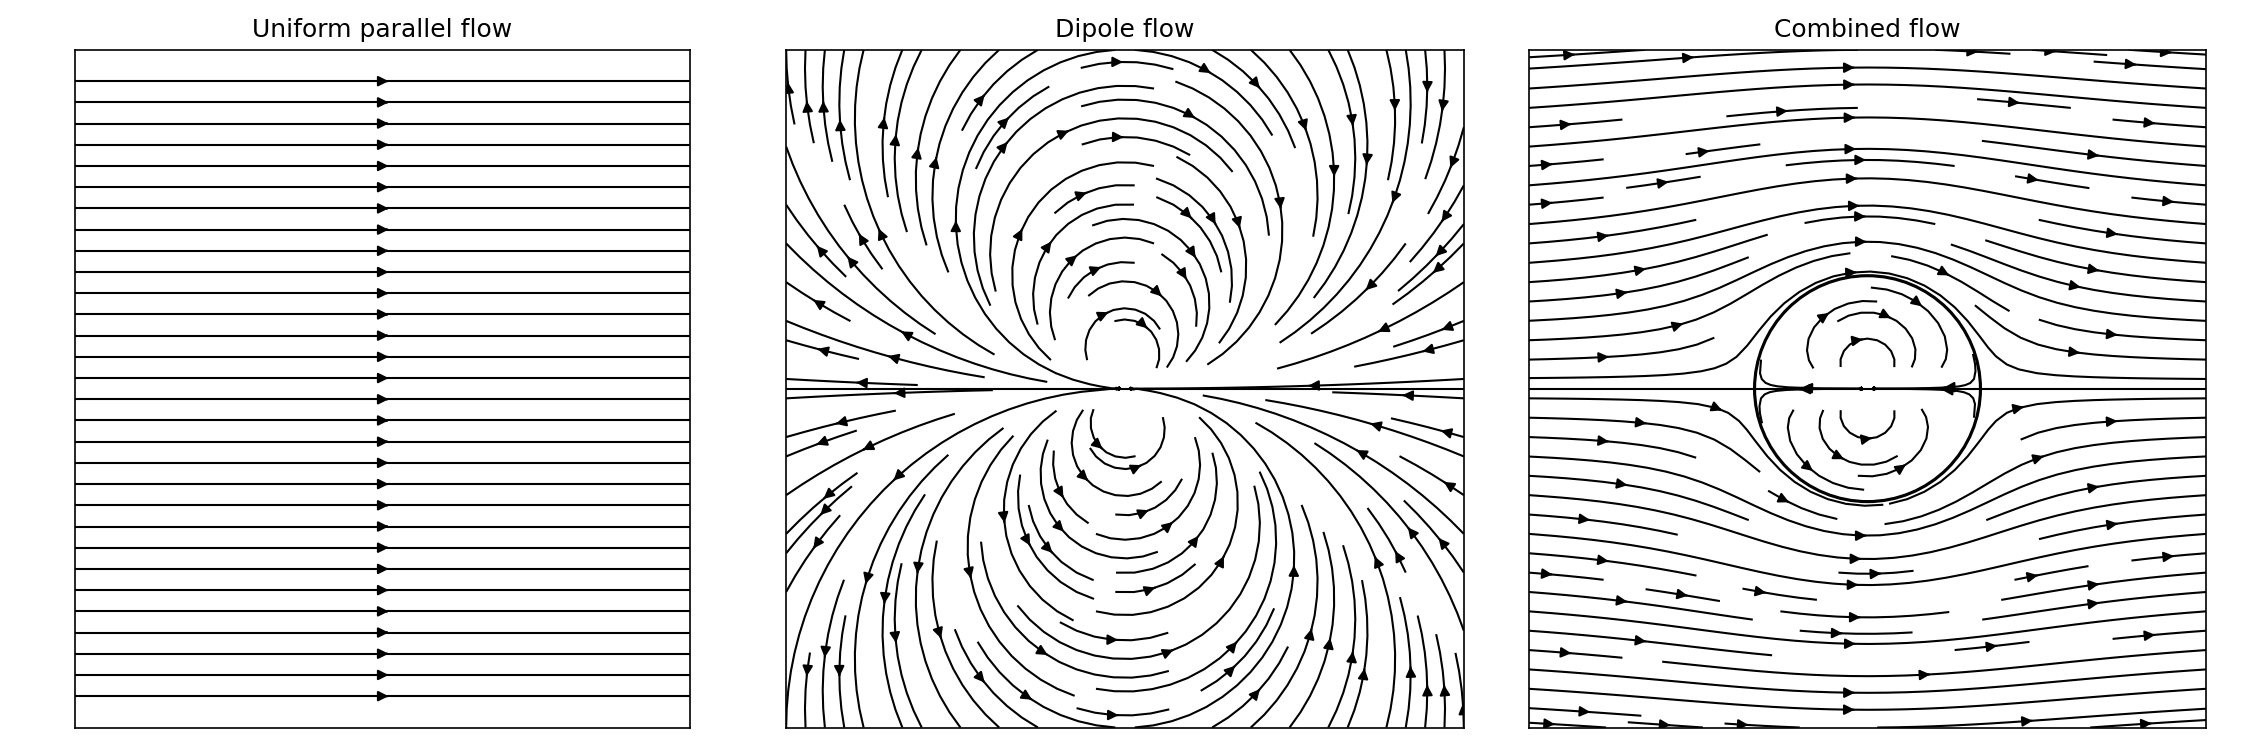
\includegraphics[width=0.85\textwidth]{images/03-combined_flow}
    \caption{Illustration of æther flow and vorticity around vortex cores.}
    \label{fig:vortexfields}
\end{figure}


\begin{description}
    \item[\textbf{Postulate I: Absolute flat space}] \hfill \\
    Space is a stationary, flat Euclidean background with a preferred frame defined by the æther at rest.\ All distances and velocities are measured in it.\ There is no intrinsic spacetime curvature; all metrics are derived from flow fields.\ (This is similar to Lorentz's original absolute frame concept, but now with a physical superfluid-like filling space~\cite{Winterberg2002-PlanckÆther}).

    \item[\textbf{Postulate II: Approximately incompressible uniform æther}] \hfill \\
    The æther behaves as an ideal fluid with zero viscosity and approximately constant mass density \textbf{$\rho^{\text{(fluid)}}_{\text{\ae}}$} in large-scale regions (analogous to superfluid helium at $T=0$). However, compressibility is permitted near vortex cores and in regions of high swirl energy, where local gradients in \textbf{$\rho^{\text{(energy)}}_{\text{\ae}}$} may develop.\ These gradients support field dynamics and mass-energy emergence.\ This scale-dependent compressibility is negligible for low-energy vortical flow but crucial in quantum-scale interactions.

    \item[\textbf{Postulate III: Vortex nodes as matter}] \hfill \\
    Matter particles are modeled as stable, topologically conserved vortex nodes.\ According to Kelvin~\cite{Kelvin1867-vortex}, an atom or fundamental particle is a quantized vortex loop or node in the æther.\ It has a well-defined core (of the order of the Planck length $l_{\textrm P}$ in radius, according to Planck-æther theories~\cite{Winterberg2002-PlanckÆther}) around which æther flows circularly.

    \item[\textbf{Postulate IV: Time as nucleus rotation}] \hfill \\
    The proper time of a particle is defined by the absolute number of full revolutions its vortex core undergoes relative to the æther.\ That is, time is an emergent internal property tied to the rotation of topological structures—not an external coordinate.

    All observers and processes exist within a shared ætheric “Now,” a globally synchronized present moment defined by the absolute rest frame of the æther.\ There is no universal ticking clock—but a common reference frame from which internal clock rates can be compared.

    Thus, two particles at different locations may experience different amounts of time passage (i.e., internal phase advance) even though they co-exist in the same \textbf{ætheric Now}.\ Time dilation arises from differences in local swirl energy, circulation speed, or core structure that influence their rotational frequencies.

    \item[\textbf{Postulate V: Thermodynamics as emergent behavior}] \hfill \\
    Temperature, entropy, and thermal fluctuations arise statistically from microscopic æther flow.\ At the base level, the æther is a perfectly inviscid, nonthermal medium.\ Dissipation and entropy are emergent, not fundamental.

    \item[\textbf{Postulate VI: Forces via vorticity}] \hfill \\
    Forces such as gravity and electromagnetism are modeled as macroscopic effects of vorticity fields in the æther.\ The gravitational limit on force $F^{\max}_{\text{gr}} = c^4 / 4 G$ emerges from ætheric flow constraints.

    \item[\textbf{Postulate VII: Vorticity Conservation}] \hfill \\
    The total vorticity $\vec{\omega}$ is conserved along flow lines unless reconnection or forcing occurs.\ This conservation governs the topology of knots and allows force transmission through analogues of Biot–Savart interactions~\cite{helmholtz1858vortices}.
\end{description}


\subsection*{Interpretation: Time as Local Rotation in a Shared Present}

In the Vortex Æther Model (VAM), time is a local property, not a global coordinate.\ The æther defines a universal present—called the \textbf{ætheric Now}—shared across all space in the preferred frame.

\begin{itemize}
    \item Each vortex accumulates proper time $\tau$ through internal revolutions.
    \item These clocks advance locally, but reference the same shared Now.
\end{itemize}

The difference between two vortex clocks is due to different angular velocities $\omega_i$:

\[
\Delta \tau = \omega_1^{-1} N_1 - \omega_2^{-1} N_2,
\]

where $N_i$ counts rotations since a common reference moment.\ This yields a purely mechanical account of proper time difference.\ \textit{In other words:} “This particle has aged more than that one” simply means “It has undergone more internal rotations relative to the ætheric present.”

\begin{remark}
\textbf{On Temporal Ontology:} We avoid the term “absolute time.” Instead, we posit a universal ætheric \emph{Now}—a globally present reference from which proper time emerges through local core rotation.
\end{remark}


\subsection*{Fundamental Constants and Relations}
The Planck time, often interpreted as the fastest meaningful tick of a quantum clock, is:
\[
    t_{\textrm P} = \sqrt{\frac{\hbar G}{c^5}} \approx 5.39\times10^{-44}\ \text{s},
\]
with $l_{\textrm P} \approx 1.62\times10^{-35}$ m the corresponding Planck length.\ In this model, such scales define core vortex radii and rotation periods.

The wave propagation (or signal) speed in the æther is given by:
\[
    c = \sqrt{\frac{B}{\rho^{\text{fluid}}_{\text{\ae}}}},
\]
where $B$ is the bulk modulus and $\rho^{\text{fluid}}_{\text{\ae}}$ is the fluid mass density.\ This governs compressional waves and sets the maximal flow velocity.

Energy density is related to fluid mass density by:
\[
    \rho^{\text{energy}}_{\text{\ae}} = \frac{1}{2} \rho^{\text{fluid}}_{\text{\ae}} c^2.
\]

Finally, the maximum force limit is:
\[
    F^{\text{max}}_{\text{gr}} = \frac{c^4}{4G} \approx 3.0 \times 10^{43}\ \text{N},
\]
which in this model represents the æther’s maximal stress capacity.
